\chapter{Previous Knowledge}
\label{cha:previous_knowledge}

Before explaining the developed path planner, various given basics have to be covered. In the following chapter genetic algorithms and their various parts will explained in-depth, for implementations and details about which of these possible functions have been chosen for the developed software, see \ref{cha:algorithm_details}. The second part will explain the vehicle and its limitations assumed in the simulation as well as the representation used, which is based on \cite{12}. Afterwards, the simulation software developed by the AG Echtzeitsysteme is introduced, part of this software is used in the program developed for this paper and will be explained in detail.

\section{About Genetic Algorithms}
\label{sec:previous_knowledge_ga}

A genetic algorithm (GA) is a search heuristic based on the "`survival of the fittest"' idea of evolutionary theory. It was developed by Holland in the 1970s \cite{15} and has since then proven itself in solving complex search problems. The idea is that the best possible solutions of an initial (usually randomly obtained) generation survive into the next generation, similar to natural selection where the strong individuals survive and get a higher chance of passing on their genes, while weaker ones die out. This process is then repeated until an optimal solution is obtained. Any given GA consists of almost the same steps, however, depending on which functions are implemented for these steps, and a number of general parameters, the resuls can drastically vary. This makes it easy to apply the GA to a large number of problems, since the basic setup is always the same and it is easy to exchange only parts of the algorithm for another one to try and get the best results. In the following the various steps of the GA are explained and several possible algorithms are given. Chapter \ref{cha:algorithm_details} explains which of these were used and why they were chosen over the other possibilities. Below is a pseudocode for a smaple GA.
\begin{verbatim}
  void function GA
    SET genCount to 0;
    initialization pop(genCount);
    evaluation pop(genCount);
    WHILE (genCount NOT EQUAL maxGenCount) do
      INCREMENT genCount;
      selection pop(genCount) from pop(genCount-1):
      crossover pop(genCount);
      mutation pop(genCount);
      evluation pop(genCount);
    ENDWHILE
\end{verbatim}

\subsection{Initialization}
\label{sec:initialization}

In order for the GA to do anything it first needs an initial generation which has to be obtained elsewhere. Unlike the following generations the initial population is usually generated randomly, but it may also be obtained from some previous computation done by another algorithm. Using a different algorithm to do preliminary computation, without letting it run so long that it would find an optimum solution, and then using the GA to optimize the solution can significantly outperform either of the two algorithms looking for an optimal solution on their own. It can however also lead to a situation where the GA has no chance of finding the optimal solution and only finds a local otipimum since the initial generation it was given did not contain enough members of the best part of the graph.
How a random population can be obtained depends heavily on the representation of the given problem within the GA, the genome. The choice of genome is one of the most important when developing a GA and also one of the hardest since there are countless possible ways to encode a problem and no real way to tell how effective a representation may be without actually implementing it. In most cases a bit string representation is chosen where every bit represents a certain possible choice within the searchspace, for example whether a certain vertex is part of the solution or not. For certain tasks other representations may be better, but in most cases binary encoding is sufficient and makes the implementations of the other functions easier.

\subsection{Evaluation}
\label{sec:evaluation}

The second step in the algorithm is the evaluation, which, like the representation of the genome, is a function that is not standarized and is, as such, hard to choose and a big factor for the performance of the GA. The evaluation function assigns a fitness rating to every genome of the given population. Every genome describes some, not necessarily possible, solution to the given problem and the fitness rating describes how good a solution that is. The rating is higher for good solutions and lower for bad ones, the exact scaling is not standarized and has to be adjusted to the given problem. For example, in some cases it might be best to remove impossible solutions from the population, in others it may be better to keep since they could still contain valuable parts for another solution. The scaling also depends on whether there is a way to know an optimal solution, in which case there would have to be a maximum fitness rating to assign to such, in other cases no maximum may be known.
The evaluation function depends on the problem to be solved and will usually require representations of the genome other than it's binary form. Functions to obtain one representaion from the other have to be implemented and some way to describe the usefulness of a solution has to be found.
Once the evaluation function is done, every genome in the currrent population should have a rating assigned to it, the consequences of this rating are defined by the other functions, mainly the selection.

\subsection{Selection}
\label{sec:selection}

The selection function takes $N$ individuals from the previous generation into the current one according to their fitness rating. The exact process of selecting and consideration of the rating depends on the algorithm employed. Since there are more algorithms, and even more variants of these algorithms, than can reasonably be explained here, we will instead concentrate on the possible functions considered or tested for our own GA. The simplest way to select $N$ individuals would be to take the $N$ best ones, this is usually not done since we want to preserve a certain randomness for two reasons. One, individuals with a low fitness rating should still have a chance to be selected since they may still contain parts of a good solution which could be extracted from the bad part by either crossover or mutation. Second, we may want good solutions to be able to be selected several times to give them a higher chance to reproduce through crossover later. The most commonly known method which fulfills both these requierements is the fitness proportionate selection\cite{16}, also known as roulette-wheel selection. It simulated a biased roulette wheel by assigning each genome a segment of the wheel, proportional in size to the genome's fitness rating, and then spinning the wheel $N$ times. This algorithm takes the fitness rating into account while still giving bad solutions a chance to be selected, albeit a low one, and also allows for good individuals to be chosen several times.  If the scaling of the fitness function is bad however this could mean that either too many bad solutions survive, because their chance was not small enough, or it could starve out the algorithm because the gap between good and bad solutions is too big and the same good-but-not-optimal solution, also known as a super-individual, is selected almost every time. Stochastic universal sampling (SUS) is an optimized version the roulette-wheel algorithm which aims to remove bias, offer minimum spread and have a low computational complexity. SUS works by selecting a random value $r$ and then choosing individuals at evenly spaced intervals instead of generating a new random value every time. This gives weaker members a better chance to be selected instead of being dominated by the better solutions.\cite{17} A different approach to selection is the tournamend selection where several individuals are chosen at random and put in a tournament with the winner being selected to the next generation. The tournament size is not fixed and can be adjusted for different needs, more competitors give weaker members a worse chance of winning, a tournament size of $1$ would be the same as random selection. A tournament can either be won by the individual with the highest rating or one chosen at random with each member having a probability proportional to their rating.

\subsection{Crossover}
\label{sec:crossover}

The crossover function chooses two individuals from the population at random and recombines their elements in a certain way to produce two new individuals. One or both of these can be kept for the new population depending on the implemenentation. Crossover is considered to be the most important search operator\cite{16}. Its results depend on the crossover operator chosen, whether one or both children are kept and the crossover rate, that is the percentage of the new population that is aquired by crossover instead of selection. The original crossover operator proposed by Holland is the \textit{one-point crossover} which chooses one position in the genome at random and switches the bits to the right of this point between the two chosen genomes. As such, one child ends up with the left part of parent one and the right part of parent two and the other child vice versa. This simple operator usually leads to inferior results \cite{18,19,20}, so \textit{multi-point crossover} operators have been introduced. These work in the same manner as the \textit{one-point crossover} operator but choose $x$ points and switch $x$ times between values from the first and second parent. Depending on implementation the crossover points may also be fixed instead of randomly chosen. Empirical studies have shown an \textit{eight-point crossover} to be optimal \cite{21,22,19}, however the \textit{two-point crossover} is the most common \cite{19}. The maximum number of crossover points is reached when the number points is equal to the number of bits in a genome, in which case we call it a \textit{uniform crossover}, which decices via fair coin toss for each bit whether it is taken from the first or second parent. This is usually done by generating a bit mask of the length of the genome instead of generating a new random boolean for each bit seperately. Other operators, which are not further explained here, include the \textit{segment crossover} \cite{19}, \textit{shuffle crossover} \cite{19} and \textit{punctuated crossover} \cite{23}.

\subsection{Mutation}
\label{sec:mutation}

The mutation operator is a simple function that, with a small chance, randomly inverts a single bit of any given genome, regardless of whether this individual has been attained by selection or mutation. The purpose of this inversion is to re-introduce certain possibilities into the population that have died out and can not be gained by crossover anymore since no member of the population has the necessary combination of bits. The mutation rate is usually very low, 0.001, 0.01 or 0.005 are common \cite{20,23,24}.

\subsection{Parameters}
\label{sec:parameters}

Once all the parts of the GA have been decided on there are only a number of parameters left to set. While there are some common practices around, most of these have to be decided by trying them out and comparing results. The most important parameters are population size, number of generations, crossover rate, mutation rate, generation gap and scaling. Population size simply determines how many individuals there are in any generation, too small a number will prevent the GA from covering the search space, too large a number will slow down computation. Population size can be anything from several hundred to several thousand and has to be tested out. Likewise, the number of generations determines how many times the algorithm runs and applies selection/crossover/mutation/evaluation, and has to be tried out. If an optimal solution is usually found after 40 or 50 iterations there is no need to continue further. This number is not necessarily set, it is a common way to determine the runtime of the algorithm, but alternative termination conditions can be set instead, for example for one individual to reach a certain fitness. The crossover rate determines the percentage of the new generation acquired by crossover instead of selection and is usually set very high. 0.6, 0.75 and 0.95 are common values \cite{20, 22,24}. Similarly, the mutation rate determines the chances of any given bit to be mutated, common values for this have already been covered in \ref{sec:mutation}. The generation gap determines how many members of the generation are replaced in the next generation, which is usually set to 1.0, meaning the entire population is replaced. Scaling is applied to the fitness rating to prevent super-individuals from scewing the results of the selection early. The exact way of scaling depends on the evaluation function and may not be necessary at all, but a sigma-truncation is common. \cite{26}

\section{About the Vehicle}
\label{sec:previous_knowledge_vehicle}

\begin{figure}[t]
\centering
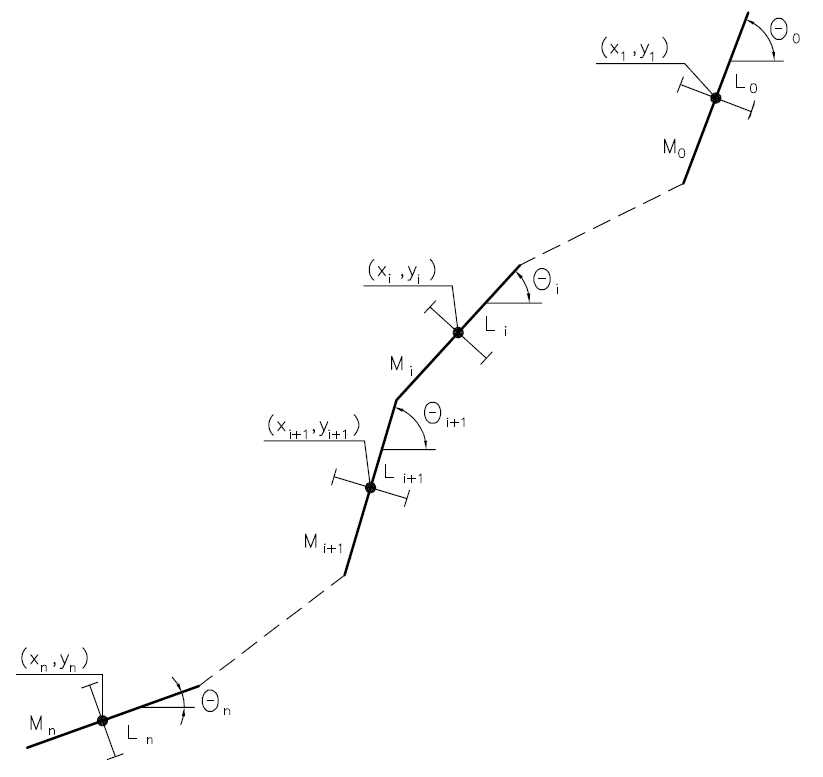
\includegraphics[width=0.75\textwidth]{./Chapters/Figures/single-track-model.png}
\caption{A vehicle in the single track model with identifiers\label{pic:single-track-model}}
\end{figure}

Our simulation software uses the control method for stable driving developed by Christian Schwarz to determine the actual path from the planned one in order to evaluate its fitness. To this end we use the same representation of the vehicle, which will be explained in the following section. The actual control software is then briefly described in \ref{sec:previous_knowledge_ezsystems}, for a complete definition and prove of stability see \cite{12}. This section also contains a short overview of nonholonomic systems, of which our vehicle is an example.
The dimensions and number of trailers of the vehicle can be freely defined in the simulation software and since no connection to an actual model is implemented yet, no further restrictions are given. The control method itself has been tested in simulation as well on a 1:16 general-2-trailer model. In order to describe the vehicle more easily and still have enough detail to achieve a correct representation, the single track vehicle model is used\cite{27}. The vehicle is first split along its flexible coupling, so any axles with rigid couplings are replaced by one virtual axis between them. The steering of the vehicle is considered to be a flexible coupling, so the tractive unit is split into 2 elements, which is why we call it a general-(n-1)-trailer if the model has n elements. Now that the vehicle is a chain of rigid parts, all wheels are replaced by points, meaning they are assumed to touch the ground in exactly one spot, and then all pairs of wheels are replaced by a single wheel in between them. \ref{pic:single-track-model} shows a general-n-trailer in its single-track model with identifiers, which are used as followed:

\begin{itemize}
	\item $(x_i,y_i)$ identifies the position of a vehicle part by the center of its axis
	\item $\theta_i$ identifies the orientation of the element
	\item $L_i$ identifies the distance from the axis to the front of the vehicle part, the front coupling point
	\item $M_i$ identifies the distance from the axis to the back of the vehicle part, the rear coupling point
\end{itemize}

The representation of the entire vehicle can be shortened by giving the positions and angles of all but the first element in relative terms. Accroding to \cite{28} the following rules hold:
\begin{itemize}
	\item $x_{i+1}=x_i-L_{i+1} cos \theta_{i+1}-M_i cos \theta_i$
	\item $y_{i+1}=y_i-L_{i+1} sin \theta_{i+1}-M_i sin \theta_i$
	\item $\alpha_{L_1}:=\theta_0-\theta_1$ is the angle of steering lock of the vehicle
	\item $\Delta \theta_{i(i+1)}:= \theta_{i+1}-\theta_i$ is the $i$-th angle of the vehicle
\end{itemize}

This leads to the complete representation of the vehicle's configuration:
\begin{center}
$\vec{g}=$
$\left(
	\begin{array}{c}
		x_1\\
		y_1\\
		\theta_1\\
		\Delta \theta_{12}\\
		\vdots\\
		\Delta \thta_{i(i+1)}\\
		\vdots\\
		\theta_{(n-2)(n-1)}\\
		\alpha_{L_1} 
	\end{array}
\right)$
\end{center}

In our program we will be using a similar representation of the vehicle, however we will give the absolute position of all elements since we need them at several points throughout drawing/computation and the effort of calculating them every time considerably outweights the cost of just saving them directly. The formulas above will be used to calculate the vehicle in the first place however.

%Possible paragraph about movemenet description

\subsection{Nonholonomic systems}
\label{sec:nonholonomic_systems}

Nonholonomic systems are a special form of kinematic systems where the degrees of freedom available are greater than the number of degrees the object can move in, which means the object cannot move along all paths that would theoretically be possible. To be more precise, this means that if a configuration space has $m$ dimensions and the vehicle has $k$ constraints such that $0<k<m$, the system is nonholonomic. It can also be defined as a system with kinematic differential constraints that are nonintegrable and cannot all be expressed as a holonomic constraint of the form $f(q,t)=0$.\cite{29,30}. A car is already a nonholonomic system as it cannot move in every direction of the plane since only one of the 2 axles are controlable and even that is limited. Our general-n-trailer has even more constraints and limitations as to how it can move in the same space and is thus also a nonholonomic system. Path-planning for such a system is more complicated due to these additional constraints, called the Pfaffian constraint, to get a proper solution. 
% Refer to possible related works here
In our case however we plan paths (more or less) at random and use the control method for stable driving to obtain a possible path from the generated one and thus make sure all constraints are fulfilled. Consequently we do not have to explicitly consider the pfaffian constraints or bring our configuration in goursat normal form, which is used to solve equations on nonholonomic systems.

\section{About the control method for stable driving}
\label{sec:about_control_method}

The EZauto software consists of many different parts for a variety of purposes, some of which wil briefly be demonstrated in \ref{sec:previous_knowledge_ezsystems}, only one of these components is implemented in our simulation software however: The control method for stable driving. \cite{12}
In our software we use paths that are created at random as an initial generation for our GA and create new paths by crossing/mutating existing genomes. Neither of the twose methods of obtaining a path has any concept of the vehicle we plan for and the limitations of the path it could take. From that is is obvious we need some way to obtain a realistic path from our desired path in order get a proper evaluation and end up with a path that is actually possible to drive. To this end we have a simulation class which implements the control method for stable driving which is called for every path before it is evaluated. This control method works similar to how humans would drive: By aiming for a certain point on the path we want to take, drive for a short distance and then adjust our steering and aim for a new point. \cite{31,32} This method works both for normal and reverse driving, only the reference point $\theta$ of the vehicle has to be adjusted. It is either the center of the rear axis of the tractive unit for normal driving or the center of the (last) trailer's axis for reverse. 
The desired path in our case is already given by either the random function or the GA so now we have to try to follow this path. To this end we choose a point on the desired path which is a "`certain distance"' away from our current position, this point is now our meeting point. Then we have to determine a circle which contains both the current position and the meeting point, this is the path we have to follow. The circle must be chosen such that the direction at the beginning, where our current position is on the circle, is the same as the direction of our $\theta$, since we can't change direction without moving.
This task now presents us with several steps: Determining the meeting point, from that the radius of the correction circle and finally the steering angle. While this method works regardless of driving direction, the calculation of the radius changes.

\subsection{The Meeting Point}
\label{sec:meeting_point}

The steps necessary for determining the meeting point depend on whether our desired path is a line or a circle, which are assumed to be the only possibilties. As shown in \cite{12} any other curve can be represented by a mixture of such lines and curves.
\ref{pic:meeting_point_linear} shows the process for a linear desired path, described by the function:
\begin{center}
$g:\mathbb{R} \to \mathbb{R}^2 , \lambda \mapsto g(\lambda ) := \vec{g_0} + \lambda \cdot \vec{h}$
\end{center}
Here $\vec{h}$ is the direction and it is assumed that $\|\vec{h}\|=1$, so the vector is normalized since its length doesn't matter. Now we try to determine the ideal point$I$, which is the point on the path our vehicle would ideally be at if there was nothing to correct. We can see $I$ in \ref{pic:meeting_point_linear} and can determine it as:
\begin{center}
$\vec{i}:= \langle \vec{p}-\vec{g_0}, \vec{h} \rangle \cdot \vec{h} + \vec{g_0}$
\end{center}
Now we can determine the meeting point $T$, denoted by the vector \vec{t}, by moving our $I$ along the desired path by $c_v>0$. The parameter $c_v$ has to be determined experimentally since it depends on the kinematic of the vehicle.
\begin{center}
$\vec{t}:=\vec{i}+c_v \cdot \vec{h} = ( \langle \vec{p} - \vec{g_0}, \vec{h} \langle + c_v) \cdot \vec{h} + \vec{g_0}$
\end{center}

\begin{figure}[h]
\centering
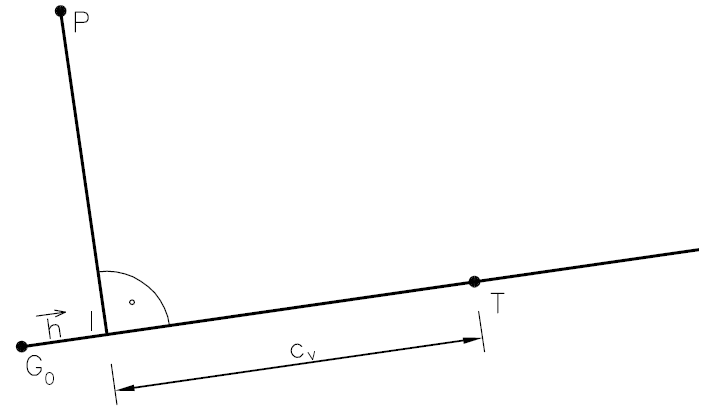
\includegraphics[width=0.75\textwidth]{./Chapters/Figures/meeting_point_linear.png}
\caption{Determining the meeting point for a linear pathpart\label{pic:meeting_point_linear}}
\end{figure}

If our desired path is a circle, illustrated in \ref{pic:meeting_point_circle}, it is given as:

\begin{center}
$k: \mathbb{R} \to \mathbb{R}^2, \varphi \mapsto k(\varphi ) := \vec{m_s}+r_s \cdot \left( \begin{array}{c} cos\varphi \\ sin \varphi \end{array} \! \right)$
\end{center}

where $|r_s|$ is the radius of the circle and its sign determines the direction: a negative sign means clockwise. Now we have to determine our ideal point $I$ again which in this case is the intersection between the center of the circle $M_s$ and our current position $P$, it is denothed by $\vec{i}$:

\begin{center}
$\vec{i}:=\frac{\vec{p}-\vec{m_s}}{\| \vec{p}-\vec{m_s}\|}$
\end{center}

Analogous to the meeting point for lines, $T$ is now determined by moving $I$, this time by rotating it around $\vec{m_s}$ by an angle with the arc length $c_v$, so the line between the ideal point and the meeting point has a length of $c_v$, just as before:

\begin{center}
$\vec{t} = 
	\begin{pmatrix}
		cos \frac{c_v}{r_s} & -sin \frac{c_v}{r_s} \\ 
		sin \frac{c_v}{r_s} & cos \frac{c_v}{r_s}
	\end{pmatrix}$
	\cdot ( \vec{i} - \vec{m_s})+\vec{m_s} 
	= \frac{r_s}{\| \vec{p} - \vec{m_s}\|}
	\begin{pmatrix}
		cos \frac{c_v}{r_s} & -sin \frac{c_v}{r_s} \\ 
		sin \frac{c_v}{r_s} & cos \frac{c_v}{r_s}
	\end{pmatrix}$
	\cdot (\vec{p} - \vec{m_s})+ \vec{m_s}
\end{center}$

\subsection{The Radius}
\label{radius}

\begin{figure}[h]
\centering
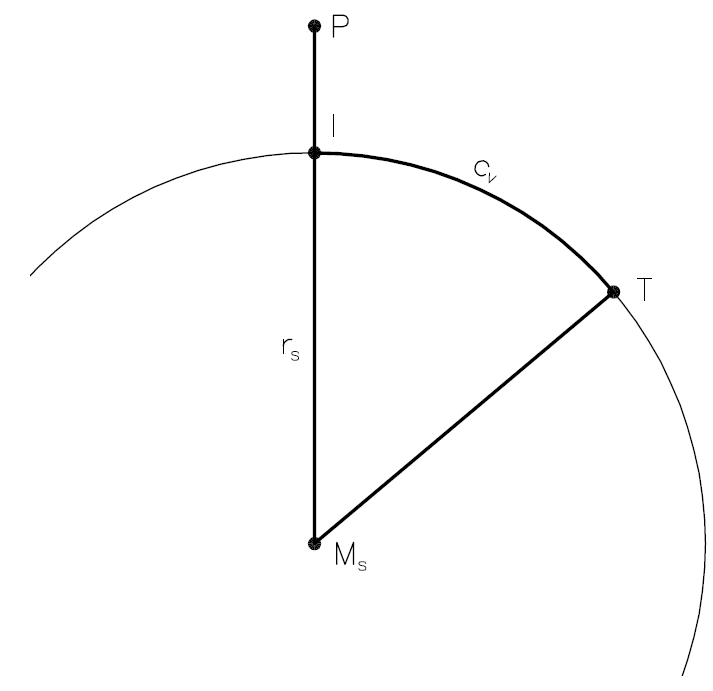
\includegraphics[width=0.75\textwidth]{./Chapters/Figures/meeting_point_circle.png}
\caption{Determining the meeting point for a circular pathpart\label{pic:meeting_point_circle}}
\end{figure}

We now have to determine the cricle we have to drive to get from our current position $P$ to our desired position $T$ determined in the last step. This circle has to be tangential to the line denoted by our current position $T$ and our current direction $\theta$, since otherwise we would be unable to follow it. Consequentially our center point lies on a line which is orthogonally to $\theta$ and runs through $P$. Also, since our desired meeting point $T$ has to be on the same circle, the line from $T$ to $P$ is a chord of the circle, so our center point lies on a perpendicular bisector of this line. See \ref{pic:correction_circle_radius} for an illustration. The vector $\vec{m_[KK}}$ denoting this point $M_{KK}$ is obtained by:

\begin{center}
$m:=
	\begin{pmatrix}
		-sin \theta \\
		cos \theta
	\end{pmatrix}
	\cdot
	\cfrac{\| \vec{p} - \vec{t} \|^2}{2 \cdot \left \langle 
	\begin{pmatrix}
		- \theta_2 \\
		\theta_1
	\end{pmatrix}
	, \vec{p} - \vec{t}
	\right \rangle
	} + \vec{p}
$
\end{center}

Accordingly, the radius is:

\begin{center}
$ r_{KK}=
\cfrac{\| \vec{p} - \vec{t} \|^2}{2 \cdot \left \langle 
	\begin{pmatrix}
		-sin \theta \\
		cos \theta
	\end{pmatrix}
	, \vec{p} - \vec{t}
	\right \rangle
	}$
\end{center}

\begin{figure}[h]
\centering
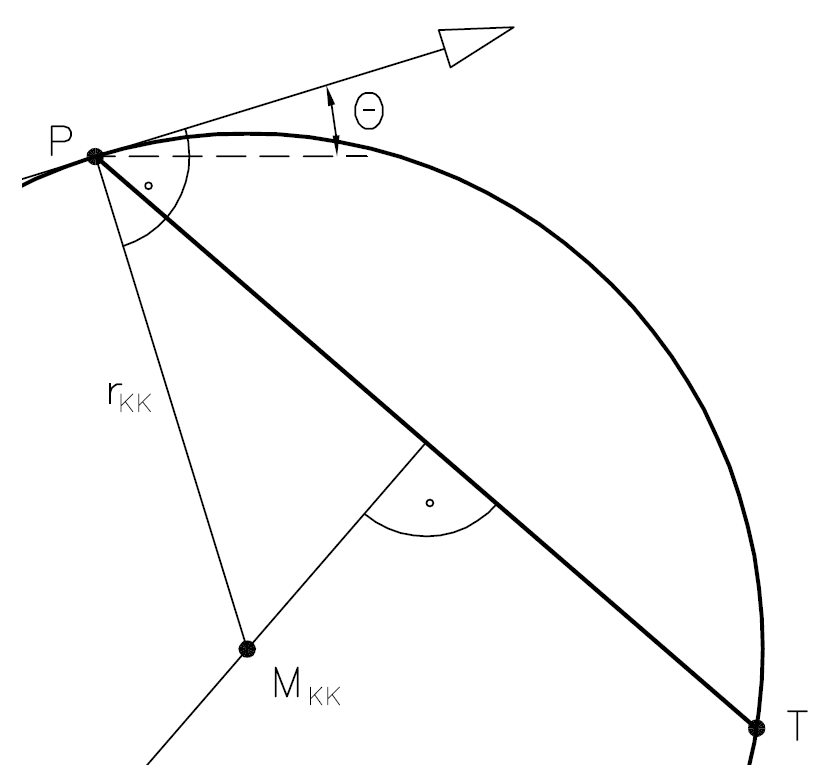
\includegraphics[width=0.75\textwidth]{./Chapters/Figures/correction_circle_radius.png}
\caption{Determining the radius of the correction circle\label{pic:correction_circle_radius}}
\end{figure}

\subsection{Calculating the steering angle}
\label{sec:calculating_steering_angle}

The process of determining the steering angle depends on the reference point of the vehicle, which, as mentioned in \ref{sec:meeting_point}, depends on the driving direction. In forward driving our reference point is the rear axis of the traction unit, $(x_1,y_1)$ (see fig. \ref{pic:vehicle_kinematic}) and our radius is $r_1$ and our steering angle is:

\begin{center}
$ \alpha_{L_1,target} = arctan \cfrac{L_2}{r_{KK}} $
\end{center}

If we are driving in reverse then our reference point is at $(x_2,y_2)$, or if there are more axles on the last one, our radius is $r_2$ and our required direction $\theta$ is:

\begin{center}
$\Delta \theta_{12,target}=-arctan \cfrac{M_1}{r_{KK} \sqrt{\cfrac{L_2^2-M^2_1}{r^2_{KK}}+1}}-arctan \cfrac{L_2}{r_{KK}}$
\end{center}

Now we have to achieve this $\Delta \theta_{12,target}$ by adjusting our steering angle, to this end we observe the behaviour of $\theta$ when adjusting the steering angle in forward driving and try to obtain a conclusion about its expected behaviour in reverse driving. From \cite{12} we know that $\theta$ converges towards a $\Delta \theta_{12,stable}$ depending on the given steering angle. We can now determine a steering angle $\alpha_{L_1,stable}$ which will lead us to our desired $\theta_12$:

\begin{center}
$\alpha_{L_1,stable}=f(\Delta \theta_12):=-arctan \cfrac{L_1 \cdot sin \Delta \theta_12}{L_2+M_1 \cdot cos \Delta \theta_12}$
\end{center}

This function $f$ is strictly monotonic decreasing in $\left[- \tfrac{\pi}{2},\tfrac{\pi}{2} \right]$ as long as $L_1, L_2, M_1 >0$. This means that our steering angle is $\alpha_{L_1,stable}=f(\Delta \theta_12)$ as long as our vehicle is in a stable state and if we want to adjust our angle by $\epsilon$ we have to set our steering to $\alpha_{L_1,stable}=f(\Delta \theta_12+\epsilon)$

% More?

\begin{figure}[h]
\centering
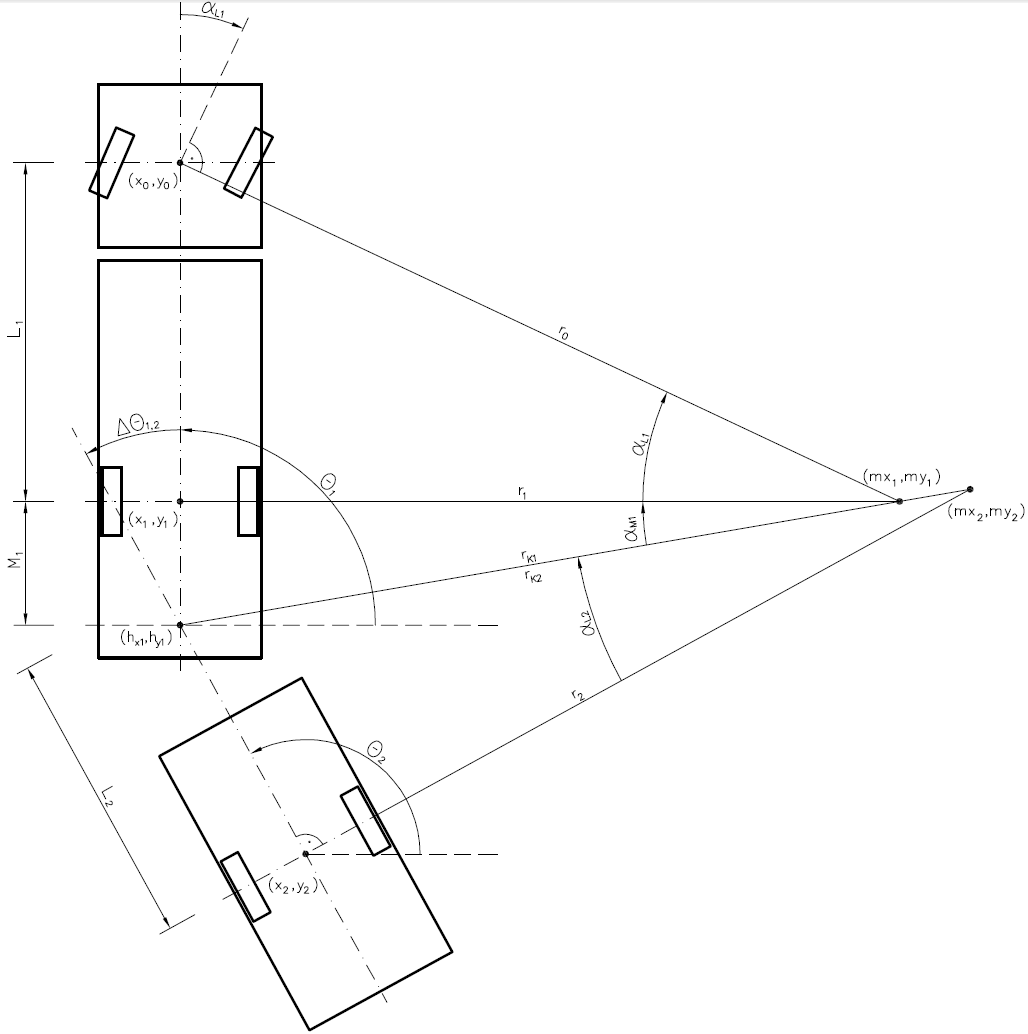
\includegraphics[width=0.75\textwidth]{./Chapters/Figures/vehicle_kinematic.png}
\caption{General-2-trailer identifiers\label{pic:vehicle_kinematic}}
\end{figure}


%\section{About the Simulation Software}
%\label{sec:previous_knowledge_ezsystems}

% Information about EZauto? Is this relevant for this paper?
